\documentclass[journal=jctcce,manuscript=article]{achemso}

\setkeys{acs}{articletitle=true,doi=true}

\usepackage[T1]{fontenc}
\usepackage{amsmath,amssymb}
\usepackage{booktabs}
\usepackage{graphicx}
\usepackage{array}
\usepackage{url}
\usepackage{xcolor}

\author{Changtian Qian}
\email{qianchangdtw@gmail.com}
\affiliation[Capital Normal University]{Department of Physics, Capital Normal University, Beijing 100048, China}

\title[QuantumChem AI]{QuantumChem AI: A Rule-Governed Electronic-Structure Workflow Platform with Grounded LLM Assistance for All-Element Atomic Clusters}

\keywords{atomic clusters, electronic structure workflows, relativistic basis-set selection, wavefunction stability, spin-symmetry scanning, Design Constitution, lanthanide superatoms}

\begin{document}
\sloppy

\begin{abstract}
Reliable quantum-chemical characterization of atomic clusters across the periodic table requires strict coupling between global configurational search, invariant isomer deduplication, element-consistent relativistic basis-set and effective core potential (ECP) assignment, open-shell spin-multiplicity scanning, Kohn--Sham wavefunction stability verification, fault-tolerant convergence escalation, and deterministic property evaluation. Conventional automated scripts commonly embed element-specific heuristics, bypass broken-symmetry stability checks, or allow large language model (LLM) wrappers to hallucinate unverified physical observables. Here, QuantumChem AI is introduced as an open-source electronic-structure workflow platform governed by an eight-article Design Constitution (C1--C8) enforced in runtime validators and continuous integration. First, a periodic-table-general YAML rule engine---verified by Python abstract syntax tree (AST) static analysis to contain zero element-symbol conditional branches---derives electron-parity-conserving spin ladders with adaptive early pruning and boundary expansion, validates Basis Set Exchange (\texttt{Gen}/\texttt{GenECP}) coverage across both ECP (\texttt{def2-SVP}/\texttt{def2-TZVP}, augmented \texttt{ma-def2-TZVP}) and all-electron scalar-relativistic (\texttt{SARC-DKH2}/\texttt{DKH2}, \texttt{ANO-RCC}) families, and disables incompatible superheavy dispersion terms ($Z > 94$). Second, a three-stage geometric deduplicator pairs distance-matrix eigenvalue fingerprinting with tri-axial principal-inertia Hungarian/Kabsch alignment to achieve $10^{-15}$~\AA\ equivalence precision in under 8~ms alongside point-group symmetry dopant enumeration. Third, a scheduler-free high-performance computing (HPC) engine executes three-section \texttt{--Link1--} refinement (\texttt{opt} $\rightarrow$ \texttt{stable=opt} $\rightarrow$ \texttt{freq}), monotonic lossless self-consistent field (SCF) escalation, and normal-mode imaginary-frequency perturbation under NUMA-aware load throttling and elastic core scaling (4 to 10--16 cores). Fourth, deterministic energetics and version-locked Multiwfn 3.8(dev) wavefunction analysis feed dual-engine Matplotlib/Origin 2024b plotting, inertia-aligned VMD/py3Dmol rendering, and \texttt{pydantic-ai} natural-language planning and read-only interpretation guarded by unit-conversion-aware numerical grounding (achieving 50/50 Chinese and 50/50 English accuracy on \texttt{deepseek-v4.1-flash}). Across 10 reference Gaussian 16 benchmarks, $\mathrm{Al_{12}Cu}$ wavefunction spectroscopy, and an autonomous 9-project, 230-job (221 Gaussian 16 runs, 1,399.78 CPU core-hours, 100\% convergence with 7 automated $4f$ repairs) study of $\mathrm{Ln@Au_5}$ ($\mathrm{Ln} = \mathrm{Gd\text{--}Lu}$), QuantumChem AI resolves a trivalent $8\mathrm{e}^-$ superatom HOMO--LUMO gap rigidity plateau (2.524--2.812~eV), core-localized $4f$ spin decoupling, and a divalent $\mathrm{Yb^{2+}}$ ($4f^{14}$, $7\mathrm{e}^-$) gap collapse and spin delocalization transition, while systematically flagging quasi-degenerate $3d$/$4f$ regimes under Article C8.
\end{abstract}

\section{Introduction}

Atomic clusters occupy the finite-size bridge between isolated atoms and condensed phases, where quantum confinement, relativistic contraction, and open-shell $d$/$f$ occupation govern shell-closure magic numbers, superatom electronic rigidity, magnetic anisotropy, and catalytic site selectivity.\cite{pyykko2002wau12,li2002wau12,jian2019pes} Determining physically faithful ground states across this chemical space demands tight coordination across potential-energy-surface (PES) exploration (e.g., ABCluster\cite{zhang2015abcluster} or tight-binding genetic algorithms\cite{bannwarth2019gfn2xtb,larsen2017ase}), rotation- and permutation-invariant isomer deduplication, consistent basis-set and relativistic treatment,\cite{weigend2005def2,pantazis2009sarc,reiher2006dkh,dolg2012ecp,pritchard2019bse} systematic spin-state scanning,\cite{cramer2009tm} wavefunction stability and normal-mode verification,\cite{bauernschmitt1996stability} fault-resilient execution on shared compute nodes,\cite{ong2013pymatgen} real-space wavefunction parsing,\cite{oboyle2008cclib,lu2012multiwfn} and reproducible visualization.\cite{humphrey1996vmd}

Despite mature software packages for individual stages, end-to-end cluster electronic-structure methodology suffers from four persistent failure modes (Table~\ref{tab:capabilities}). First, element-specific fragmentation arises when workflow scripts hardcode functionals, basis sets, or trial spin multiplicities for narrow families such as pure gold or silicon clusters, breaking silently or introducing methodological discontinuities when extended to open-shell $3d$/$5d$ transition metals, bimetallic alloys, or $4f$ lanthanide clusters. Second, silent electronic-structure artifacts accumulate whenever workflows omit strict theory-level matching between clusters and atomic/ionic references, skip $\langle S^2 \rangle$ spin-contamination auditing, or neglect \texttt{stable=opt} Kohn--Sham stability checks\cite{bauernschmitt1996stability} and broken-symmetry convergence protocols. Third, shared-cluster execution without centralized queue managers frequently triggers cross-socket NUMA contention, whereas Gaussian SCF oscillations (\texttt{L502}), optimization cycle limits (\texttt{L9999}), and saddle-point imaginary modes require automated, basis-tail-preserving recovery. Fourth, exposing general-purpose large language models (LLMs) directly to raw computational logs invites fabricated energies, frontier gaps, and structural parameters.\cite{bran2024chemcrow,boiko2023coscientist}

\begin{table}[htbp]
  \centering
  \caption{Methodological Capabilities of QuantumChem AI Compared with Conventional Cluster Scripts and General High-Throughput Material Frameworks}
  \label{tab:capabilities}
  \footnotesize
  \begin{tabular}{>{\raggedright\arraybackslash}p{2.4cm} >{\raggedright\arraybackslash}p{3.6cm} >{\raggedright\arraybackslash}p{3.7cm} >{\raggedright\arraybackslash}p{4.3cm}}
    \toprule
    Methodology Dimension & Conventional Cluster Scripts & General High-Throughput Frameworks & QuantumChem AI (This Work) \\
    \midrule
    Elemental generality & Hardcoded to narrow chemical families & Focused on periodic crystals and bulk solids & Full periodic table (H--Rn \& $4f$/$5f$); AST-verified zero element branches \\
    Relativistic \& basis rules & Manual basis/ECP pasting; prone to mismatch & Pseudopotential tables for plane waves & BSE \texttt{Gen}/\texttt{GenECP} coverage checks; \texttt{def2}, \texttt{ma-def2}, \texttt{SARC-DKH2}/\texttt{DKH2} support \\
    Spin \& stability rigor & Manual trial multiplicities; \texttt{stable=opt} omitted & Periodic spin polarization; molecular \texttt{--Link1--} rare & Parity conservation + adaptive early-stop/expansion + 3-section \texttt{--Link1--} \\
    Shared-HPC recovery & Manual \texttt{nohup}/\texttt{screen}; prone to node overload & Dependent on Slurm/PBS queue managers & NUMA probing + load throttling + elastic core scaling + lossless $4f$/tail repair \\
    Analysis \& AI grounding & Manual Excel/Origin/VMD; ungrounded chat & Minimal validated planning/analysis coupling & Version-locked Multiwfn + dual-engine plots + \texttt{pydantic-ai} numerical guard \\
    \bottomrule
  \end{tabular}
\end{table}

This work addresses these four challenges with QuantumChem AI, an open-source computational workflow platform built over established libraries (ASE,\cite{larsen2017ase} pymatgen/custodian,\cite{ong2013pymatgen} Basis Set Exchange,\cite{pritchard2019bse} cclib,\cite{oboyle2008cclib} and Multiwfn\cite{lu2012multiwfn}) and governed by an eight-article Design Constitution (C1--C8). By separating declarative periodic-table and electronic-structure rules from execution plumbing and enforcing deterministic numerical grounding across both HPC pipelines and LLM interfaces, QuantumChem AI transforms natural-language or programmatic study specifications into verified minima, wavefunction descriptors, and publication-ready deliverables.

\section{Workflow Architecture and Design Constitution}

\subsection{Eight-Article Design Constitution (C1--C8)}

Drawing on explicit rule-based governance,\cite{bai2022constitutional} QuantumChem AI codifies eight operational invariants (C1--C8) enforced continuously at both static test-suite gates and runtime execution boundaries:

\begin{description}
  \item[C1 (Numerical Determinism)] Total energies, relative isomer stabilities, HOMO--LUMO gaps, binding energies, spin expectation values, and charge/spin populations are evaluated exclusively by deterministic Python, cclib, and Multiwfn routines and stored in structured databases. Natural-language components never compute or estimate observables; every AI analytical statement must pass a deterministic numerical grounding guard.
  \item[C2 (Zero Element-Symbol Hardcoding)] Conditional branches referencing explicit chemical symbols (e.g., \texttt{if symbol == "Au"}) are forbidden across \texttt{src/}. Rules operate solely on intrinsic periodic-table attributes (atomic number $Z$, group, period, block $s/p/d/f$, and valence subshell occupancy), verified on every test run by an abstract syntax tree (AST) scanner (\texttt{test\_axiom\_no\_\allowbreak{}element\_branches.py}).
  \item[C3 (Single-Source Rules \& Decision Provenance)] Theory tiers, dispersion corrections, multiplicity caps, charge templates, and study recipes reside solely in \texttt{src/qcai/knowledge/rules/*.yaml} paired with physical rationales and literature citations. Every emitted \texttt{Decision} object records its rule identifier and any user override.
  \item[C4 (Theory-Level Consistency)] Comparative energetic observables---binding energy ($E_b$), second-order energy difference ($\Delta_2 E$), fragmentation energy ($E_f$), embedding energy ($E_{\text{emb}}$), substitution energy ($E_{\text{sub}}$), mixing excess energy ($\Delta$), and vertical/adiabatic detachment energies (VDE/ADE)---enforce identical functionals, dispersion models, basis sets, and ECP definitions across clusters, isolated atoms, and ionic states.
  \item[C5 (Data--Rendering Decoupling)] Analysis modules emit tool-agnostic \texttt{FigureSpec} payloads consumed identically by \texttt{MatplotlibRenderer} and \texttt{OriginRenderer}, ensuring strict numerical equivalence between quick previews and editable OriginLab \texttt{.opju} workbooks.
  \item[C6 (Credential Isolation \& Zero Echo)] SSH host credentials, private paths, and API keys never enter version control, logs, diagnostic archives, or LLM prompt contexts; API keys are stored exclusively in the operating-system keyring.
  \item[C7 (Shared-Cluster Courtesy \& Idempotent Recovery)] Pipeline state persists in SQLite for pause/resume reconciliation across network interruptions, while live server probing halts new job submissions whenever competing users saturate host compute resources.
  \item[C8 (Automatic Defect Surfacing \& Multireference Advisories)] Imaginary vibrational modes, Kohn--Sham wavefunction instabilities, $\langle S^2 \rangle$ spin contamination, custodian fault-recovery histories, and $f$-block static-correlation advisories aggregate automatically into \texttt{ProjectSummary.all\_issues}, propagating explicitly to reports, web views, and AI summaries.
\end{description}

\subsection{Five-Layer Architecture and S0--S7 Multi-Fidelity Funnel}

As shown in Figure~\ref{fig:arch}a, QuantumChem AI separates concerns across five deterministic layers linked by typed Pydantic contracts (\texttt{ResearchRequest}, \texttt{CalcPlan}, \texttt{JobSpec}, and \texttt{CalcResult}), while six generic plugin registries (\texttt{Registry[T]}) abstract external backends: \texttt{QCPROGRAMS} (Gaussian 16,\cite{frisch2019g16} extensible to ORCA/CP2K), \texttt{GENERATORS} (coordinate import, ABCluster, Molclus, ASE-GA), \texttt{RENDERERS} (Matplotlib, Origin 2024b), \texttt{RUNNERS} (SSH \texttt{DirectRunner}, \texttt{MockRunner}), \texttt{LLMS} (\texttt{DeepSeekLLMProvider}), and \texttt{PROFILES} (\texttt{ClusterProfile}). Figure~\ref{fig:arch}b illustrates the constitutional closed-loop LLM controllers governing planning and read-only interpretation, and Figure~\ref{fig:arch}c summarizes the idempotent S0--S7 multi-fidelity funnel orchestrated by \texttt{PipelineWorker}:

\begin{figure}[htbp]
  \centering
  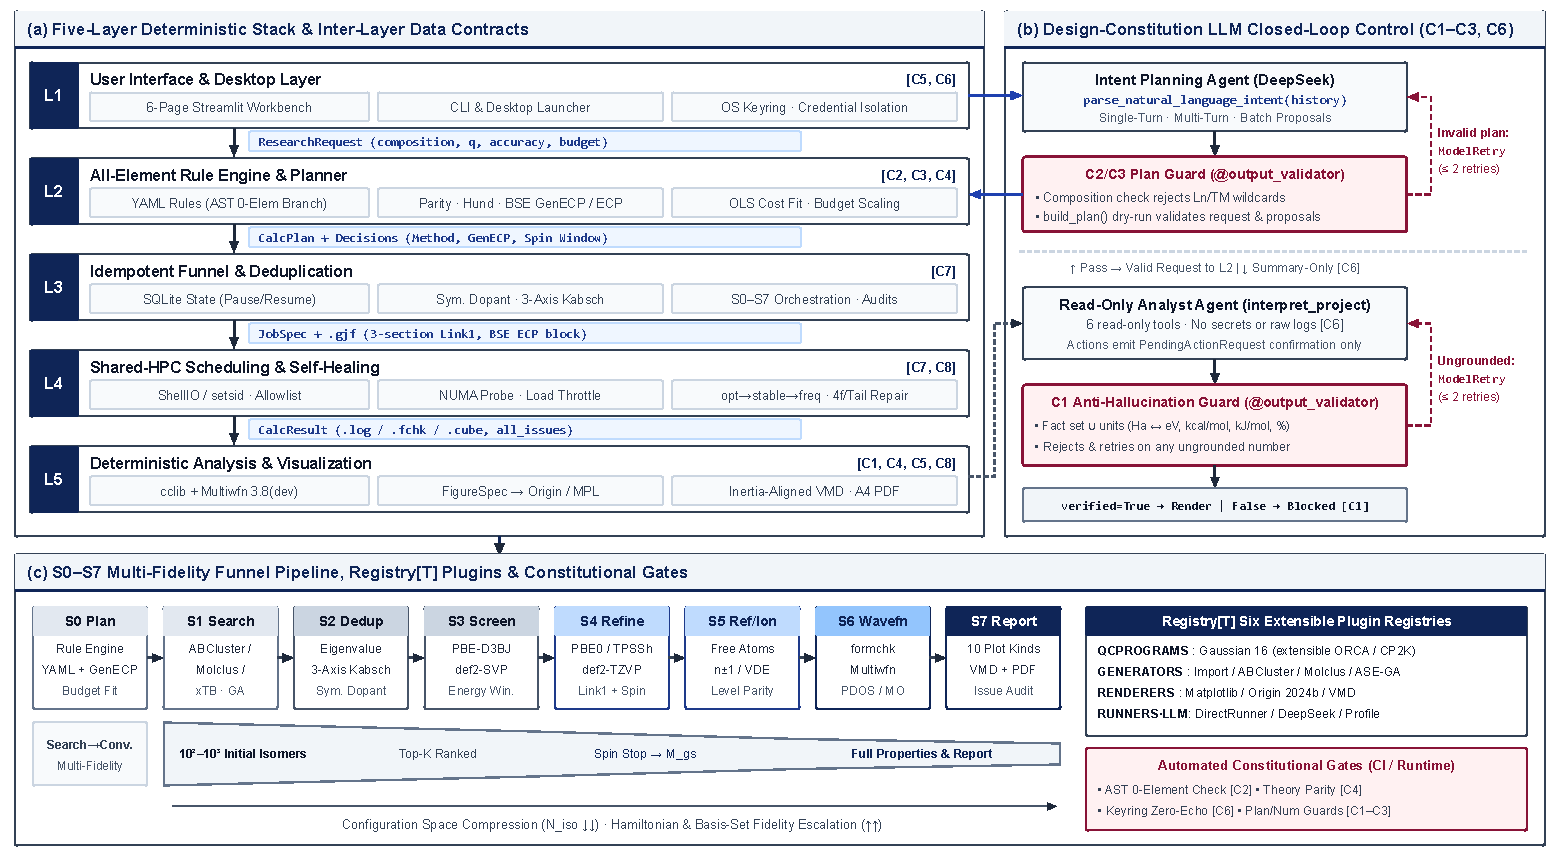
\includegraphics[width=\textwidth]{figures/fig1.pdf}
  \caption{QuantumChem AI electronic-structure workflow architecture and Design Constitution enforcement: (a) five-layer deterministic software stack and Pydantic data contracts; (b) Design-Constitution-governed LLM planning and read-only numerical anti-hallucination loop (C1--C3, C6); (c) S0--S7 multi-fidelity configurational funnel, \texttt{Registry[T]} plugin interfaces, and runtime/CI constitutional gates.}
  \label{fig:arch}
\end{figure}

\begin{description}
  \item[S0 (Planning \& Reference Atoms)] Resolves \texttt{ResearchRequest} via the YAML rule engine into an auditable \texttt{CalcPlan} and dispatches level-matched isolated atomic reference jobs.
  \item[S1 (Global Structural Search)] Prioritizes user-supplied coordinates, ABCluster (\texttt{isomer} + GFN2-xTB), Molclus, or an automated \texttt{ase-ga} + \texttt{tblite} GFN2-xTB fallback, combined with symmetry-unique dopant enumeration for alloy and endohedral clusters.
  \item[S2 (Geometric Deduplication \& Windowing)] Filters high-energy and spatially equivalent isomers, advancing the top $K$ distinct representatives to DFT.
  \item[S3 (Coarse DFT Screening)] Optimizes and ranks candidate geometries and trial spin states at PBE-D3BJ/def2-SVP\cite{perdew1996pbe,grimme2011d3bj,weigend2005def2} (or PBE0-D3BJ/def2-SVP under the high-accuracy tier).
  \item[S4 (High-Fidelity Refinement \& Spin Scan)] Refines surviving isomers at hybrid or meta-hybrid triple-$\zeta$ DFT (PBE0-D3BJ/def2-TZVP\cite{adamo1999pbe0} or TPSSh-D3BJ/def2-TZVP\cite{staroverov2003tpssh}) under the three-section \texttt{--Link1--} protocol (\texttt{opt} $\rightarrow$ \texttt{stable=opt} $\rightarrow$ \texttt{freq}) with adaptive multiplicity pruning.
  \item[S5 (Neighbor \& Vertical Detachment States)] Evaluates level-matched $n \pm 1$ clusters and vertical/adiabatic ionic states (VDE/ADE/VIP/VEA).\cite{jian2019pes}
  \item[S6 (Wavefunction Post-Processing)] Converts checkpoints via \texttt{formchk}, executes version-locked Multiwfn 3.8(dev)\cite{lu2012multiwfn} scripts for Hirshfeld/ADCH charges, atomic spin populations, projected density of states (PDOS), and frontier orbital compositions, and writes \texttt{.cube} spin/MO grids via \texttt{cubegen}.
  \item[S7 (Synthesis, Visualization \& Reporting)] Evaluates deterministic observables, renders 10 classes of 2D figures and inertia-aligned 3D views, and compiles A4 HTML/PDF reports.
\end{description}

\section{Electronic-Structure Methodology and Core Algorithms}

\subsection{Relativistic Basis-Set Selection Rules and Zero-Hardcoding Rule Engine}

The planning and input-generation layers (\texttt{src/qcai/planner/} and \texttt{src/qcai/programs/gaussian/writer.py}) transform arbitrary compositions $\{Z_i\}$ and net charge $q$ into self-consistent Gaussian 16 inputs using periodic attributes and physical conservation laws without element-symbol branching:

\begin{description}
  \item[Relativistic Basis-Set Coverage \& \texttt{Gen}/\texttt{GenECP} Resolution] Prior to input emission, \texttt{check\_basis\_coverage()} queries Basis Set Exchange (\texttt{bse})\cite{pritchard2019bse} metadata across every element in the cluster. For standard built-in Karlsruhe sets (\texttt{def2-SVP}, \texttt{def2-TZVP}, \texttt{def2-QZVP}, \texttt{def2-TZVPP})\cite{weigend2005def2} and \texttt{LANL2DZ}, \texttt{resolve\_gaussian\_basis()} checks Gaussian 16's built-in element tables ($Z \in [1,57] \cup [72,86]$ for \texttt{def2}). Whenever a cluster contains elements absent from Gaussian 16's native tables---such as $4f$ lanthanides $\mathrm{Ce\text{--}Lu}$, or when diffuse minimally augmented basis sets (\texttt{ma-def2-TZVP})\cite{zheng2011madef2} or per-element mixed basis dictionaries are specified---the writer exports explicit \texttt{gaussian94}-formatted basis and pseudopotential blocks directly from BSE, selecting the \texttt{GenECP} route keyword whenever \texttt{-ECP} definitions are present and \texttt{Gen} for all-electron specifications. For scalar-relativistic all-electron workflows---such as second-order Douglas--Kroll--Hess (\texttt{DKH2})\cite{reiher2006dkh} calculations invoked via \texttt{CalcSpec.extra\_keywords}---the preferred fallback registry includes all-electron scalar-relativistic \texttt{SARC-DKH2} (\texttt{SARC-DKH-TZVP} family)\cite{pantazis2009sarc} and \texttt{ANO-RCC} basis sets, automatically verified against BSE and emitted as \texttt{Gen} blocks. Empirical dispersion keywords (\texttt{GD3}/\texttt{GD3BJ})\cite{grimme2011d3bj} are automatically suppressed when any element exceeds Gaussian 16's $Z = 94$ (\texttt{Pu}) parameterization bound (verified in unit tests on $\mathrm{Am}$ with \texttt{SARC-DKH2}), while unrestricted (\texttt{U}) functional prefixes and \texttt{nosymm} are enforced for open-shell and symmetry-breaking cluster optimizations.
  \item[Electron Parity \& Hund-Rule Atomic Multiplicities] Given total electron count $N_e = \sum_i Z_i - q$, permissible spin multiplicities $M = 2S + 1$ satisfy $(N_e + M) \bmod 2 = 1$ with $M - 1 \le N_e$. Isolated atomic reference multiplicities query ASE ground-state magnetic moments and fall back to Hund-rule subshell fillings from \texttt{pymatgen} for lanthanides and heavy elements.
  \item[Adaptive Multiplicity Scan with Early Stopping \& Boundary Expansion] Initial spin-scan windows scale by block ($d$/$f$ cap $M_{\max} \le 12$, main-group cap $\le 6$) and converge dynamically via Algorithm~1 (Table~\ref{tab:alg1}): high-spin branches prune once two consecutive multiplicities exceed the running minimum $E_{\min}$ by $\Delta E_{\text{stop}} = 0.50$~eV, whereas boundary minima trigger automatic expansion in steps of $\Delta M = 2$.
  \item[Size Scaling \& Cost-Budget Contraction] Rule \texttt{rule.size.basis\_downgrade} scales refinement basis sets to \texttt{def2-SVP} and caps candidates at $K=5$ above 20 atoms, while an ordinary least-squares runtime model calibrates wall-clock scaling and contracts $K$ deterministically under user time budgets.
\end{description}

\begin{table}[htbp]
  \centering
  \caption{Algorithm 1: Adaptive Spin-Multiplicity Scan with Early Stopping and Boundary Expansion in Stage S4}
  \label{tab:alg1}
  \small
  \begin{tabular}{p{14.8cm}}
    \toprule
    Input: Pre-screened geometry $G$, electron count $N_e$, initial window $\mathcal{M}_0 = [M_{\min}, \dots, M_{\max}]$, threshold $\Delta E_{\text{stop}} = 0.50$~eV. \\
    Output: Converged spin-ladder results $\mathcal{R}$ and ground-state multiplicity $M_{\text{gs}}$. \\
    \midrule
    1:\quad Initialize $\mathcal{M}$ retaining only states with $(N_e + M) \bmod 2 = 1$ and $M - 1 \le N_e$; enqueue initial batch. \\
    2:\quad \textsc{while} active jobs remain or boundary expansion is triggered \textsc{do} \\
    3:\quad \hspace{1.2em} Collect normal-termination energies $E(M)$; set $E_{\min} \leftarrow \min_M E(M)$ and $M_{\text{best}} \leftarrow \arg\min_M E(M)$. \\
    4:\quad \hspace{1.2em} \textsc{if} two consecutive states $M > M_{\text{best}}$ satisfy $E(M) - E_{\min} > \Delta E_{\text{stop}}$ \textsc{then} \\
    5:\quad \hspace{2.4em} Cancel higher-spin queued jobs (early-stop pruning) and record \texttt{Decision}. \\
    6:\quad \hspace{1.2em} \textsc{if} $M_{\text{best}} = \min(\mathcal{M})$ and $M_{\text{best}} > 2$ \textsc{then} enqueue $M_{\text{next}} = M_{\text{best}} - 2$. \\
    7:\quad \hspace{1.2em} \textsc{else if} $M_{\text{best}} = \max(\mathcal{M})$ \textsc{then} enqueue $M_{\text{next}} = M_{\text{best}} + 2$. \\
    8:\quad \textsc{return} $M_{\text{gs}} = \arg\min_M E(M)$ and complete ladder $\mathcal{R}$. \\
    \bottomrule
  \end{tabular}
\end{table}

\subsection{Symmetry Dopant Enumeration and Three-Stage Geometric Deduplication}

For doped and bimetallic clusters (\texttt{src/qcai/structure/dopant\_sites.py}), \texttt{PointGroupAnalyzer}\cite{ong2013pymatgen} partitions host atomic coordinates into symmetry-equivalent orbits, emitting one representative per orbit for single substitution (e.g., 1 trial site for $O_h$ or $I_h$ hosts) and symmetry-canonicalized tuples for multi-site doping alongside centroid cavity coordinates for endohedral doping.

Conventional single-axis alignment in \texttt{pymatgen.HungarianOrderMatcher} produces spurious $1.7\text{--}1.9$~\AA\ RMSDs on rotated clusters with near-degenerate principal moments of inertia. The three-stage invariant deduplicator (\texttt{src/qcai/structure/dedup.py}) eliminates these false negatives:
\begin{enumerate}
  \item Distance-matrix eigenvalue fingerprinting computes $\mathcal{O}(N^3)$ sorted eigenspectra of pairwise interatomic distance matrices within the energy window for exact rotation-, translation-, and permutation-invariant pre-filtering.
  \item Tri-axial principal-inertia alignment maps structures to mass-weighted principal-inertia frames across all four proper right-handed sign flips, solves per-element optimal atom assignment via the Hungarian algorithm\cite{kuhn1955hungarian} (\texttt{scipy.optimize.linear\_sum\_assignment}), and minimizes Cartesian deviation via Kabsch rotation.\cite{kabsch1976}
  \item Degenerate-axis fallback invokes \texttt{BruteForceOrderMatcher} ($N \le 7$) or \texttt{GeneticOrderMatcher} ($N \le 24$) whenever borderline high-symmetry polyhedra exceed the initial RMSD cutoff ($0.25$~\AA). Across 6--38 atom tests, rotated, translated, and permuted duplicates converge to $10^{-15}$~\AA\ RMSD in $< 8$~ms per comparison.
\end{enumerate}

\subsection{Wavefunction Stability Protocols, SCF Escalation, and Shared-HPC Scheduling}

Because Gaussian 16 rejects co-located \texttt{opt} and \texttt{stable=opt} directives on a single route card (\texttt{Illegal IType}), \texttt{write\_gaussian\_input()} decomposes refinement tasks into three sequential \texttt{--Link1--} sections: geometry optimization (\texttt{opt}), Kohn--Sham stability optimization (\texttt{stable=opt geom=allcheck guess=read}), and harmonic frequency verification (\texttt{freq geom=allcheck guess=read}), substituting \texttt{chkbasis} on follow-up steps whenever the primary section uses \texttt{Gen} or \texttt{GenECP}. To accommodate single-section \texttt{stable=opt} logs where Gaussian prints an initial instability prior to re-optimization, the parser tracks stability flags per \texttt{--Link1--} section so the final stabilized state governs \texttt{CalcResult.stable}.

On shared Linux servers without centralized Slurm/PBS queues (\texttt{src/qcai/remote/} and \texttt{src/qcai\_remote/}), the execution engine pairs path-confined Fabric SSH transport with a hardened \texttt{custodian} error-recovery loop:
\begin{itemize}
  \item \texttt{qcai\_remote/probe.py} fuses \texttt{psutil}, \texttt{lscpu -J}, and \texttt{ps -eo user,pcpu,comm} to probe NUMA socket boundaries, available RAM, and competing user CPU load. \texttt{ResourceManager} pins jobs within single NUMA nodes, pauses submissions when host resources are congested, and dynamically scales queued S4 jobs from 4 to 10--16 cores (adjusting \texttt{\%mem} proportionally) as earlier batches drain.
  \item Keepalive heartbeats (30~s), automatic channel reconnection, stdin isolation, stale-checkpoint exclusion, and immediate post-exit \texttt{status.json} synchronization eliminate check-vs-exit race conditions.
  \item Monotonic SCF escalation (\texttt{upgrade\_scf\_route\_line()}) steps non-convergent open-shell $d$/$f$ jobs along three increasingly damped protocols without repeating exhausted settings: \texttt{scf=(xqc,maxcycle=512,vshift=500,fermi,novaracc)} $\rightarrow$ \texttt{scf=(xqc,maxcycle=512,vshift=800,fermi,novaracc,ndamp=30)} $\rightarrow$ \texttt{scf=(maxcycle=512,vshift=1000,fermi,novaracc,ndamp=40)}.
  \item Lossless tail restoration (\texttt{restore\_gjf\_tail\_if\_lost()}) preserves \texttt{/GenECP} route tags and trailing BSE basis/ECP/\texttt{--Link1--} blocks whenever upstream rewrites truncate them, while \texttt{ImaginaryFreqHandler} (\texttt{step\_scale=0.25} along the first imaginary normal mode) and \texttt{InstabilityHandler} drive saddle points and unstable wavefunctions to verified local minima.
\end{itemize}

\subsection{Deterministic Energetics, Multiwfn Parsing, and Grounded LLM Control}

Under Articles C1 and C4, \texttt{src/qcai/analysis/} computes all cluster observables via unit-tested equations:
\begin{align}
  E_b &= \frac{\sum_k n_k E(\text{atom}_k) - E(\text{cluster})}{N} \label{eq:eb} \\
  \Delta_2 E(n) &= E(n+1) + E(n-1) - 2E(n) \label{eq:d2e} \\
  E_f &= E(A) + E(B) - E(AB) \label{eq:ef} \\
  E_{\text{emb}} &= E(\text{Host}) + E(\text{Dopant}) - E(\text{Host+Dopant}) \label{eq:eemb} \\
  E_{\text{sub}} &= E(\text{Host}_{n-1}D) + E(\text{Host}_{\text{atom}}) - E(\text{Host}_n) - E(D) \label{eq:esub} \\
  \Delta(A_m B_n) &= E(A_m B_n) - \frac{m}{m+n}E(A_{m+n}) - \frac{n}{m+n}E(B_{m+n}) \label{eq:mix} \\
  \text{VDE} &= E_{\text{neu}}(\mathbf{R}_{\text{an}}) - E_{\text{an}}(\mathbf{R}_{\text{an}}), \qquad
  \text{ADE} = E_{\text{neu}}(\mathbf{R}_{\text{neu}}) - E_{\text{an}}(\mathbf{R}_{\text{an}}) \label{eq:pes} \\
  f_D &= \frac{\sum_{i \in D}|s_i|}{\sum_{\text{all } j}|s_j|} \label{eq:fd}
\end{align}
Jellium valence-electron counts flag closed-shell superatom closures ($2, 8, 18, 20, 34, 40, 58, 92$), while spin contamination triggers \texttt{SPIN\_CONTAMINATION} in \texttt{ProjectSummary.all\_issues} whenever $|\langle S^2 \rangle - S(S+1)| > 0.10\,S(S+1)$ (or $|\langle S^2 \rangle| > 0.10$ for singlets). Under Article C8, this spin-contamination audit works in tandem with \texttt{rule.f\_block.experimental\_warning} and \texttt{WAVEFUNCTION\_UNSTABLE} to establish a principled single-reference boundary: systems showing minimal spin contamination and confirmed \texttt{stable=opt} minima are validated within broken-symmetry hybrid DFT, whereas quasi-degenerate $3d$/$4f$ manifolds exhibiting persistent SCF non-convergence or elevated $\langle S^2 \rangle$ deviations are flagged explicitly for multireference (e.g., CASSCF/CASPT2) or spin-orbit treatment.

To guard against menu shifts across Multiwfn releases, \texttt{src/qcai/programs/multiwfn/} verifies the executable banner against \texttt{Version 3.8(dev) (2025-Mar-10)}, raising \texttt{MultiwfnVersionError} on mismatch. Regex preprocessing (\texttt{(?<=\textbackslash d)-}) splits fixed-width Fortran negative-sign concatenations in \texttt{DOS\_curve.txt}, enabling exact extraction of Hirshfeld/ADCH charges, atomic spin populations, element- and angular-momentum-resolved PDOS, and frontier orbital compositions. Under Article C5, \texttt{FigureSpec} dispatches 10 plot classes identically to Matplotlib and Origin 2024b (producing PNG, SVG, and editable \texttt{.opju} workbooks), while \texttt{align\_cluster\_principal\_axes} locks interactive \texttt{py3Dmol} and ray-traced VMD (\texttt{TachyonInternal}) scenes to a common principal-inertia frame prior to A4 PDF compilation.

In \texttt{src/qcai/ai/}, two decoupled \texttt{pydantic-ai} agents enforce constitutional bounds: (1) an intent-to-plan parser that rejects generic element wildcards (\texttt{Ln}, \texttt{TM}, \texttt{M}) and executes \texttt{build\_plan()} as an output validator on every direct request and family-level \texttt{ProposedPlan} (issuing automatic schema-repair retries on constraint errors), and (2) a read-only analytical interpreter limited to six non-mutating query tools plus a confirmation-request tool. Its grounding validator (\texttt{src/qcai/ai/guard.py}) extracts all quantitative claims and verifies them against observed fact numbers expanded across Hartree $\leftrightarrow$ eV ($27.211386$~eV/Ha), kcal/mol ($627.509474$), kJ/mol ($2625.49964$), and percentage conversions, blocking unverified outputs after retry exhaustion.

\section{Validation and Production Case Studies}

\subsection{Ten Reference Gaussian 16 Benchmarks}

Ten reference Gaussian 16 calculations spanning $s$-block ($\mathrm{Na_6}$), $p$-block superatoms ($\mathrm{Al_{13}^-}$), $3d$ high-spin ($\mathrm{Fe_4}$), $5d$ endohedral \texttt{GenECP} ($\mathrm{W@Au_{12}}$), bimetallic alloys ($\mathrm{Cu_3Ag_3}$), Jahn--Teller doped open-shell clusters ($\mathrm{Al_{12}Cu}$), two-section \texttt{Link1} stability checks, and four intentional fault-injection scenarios were executed on Linux compute nodes via \texttt{DirectRunner} and archived in \texttt{tests/data/golden/}. Table~\ref{tab:golden} summarizes parsed observables and server-side \texttt{custodian} outcomes; Figure~\ref{fig:vmd} shows inertia-aligned VMD 3D renderings for the six converged chemical clusters, and Figure~\ref{fig:gaps} compares their HOMO--LUMO gaps.

\begin{table}[htbp]
  \centering
  \caption{Parsed Observables and Server-Side \texttt{custodian} Recovery Outcomes for Ten Reference Gaussian 16 Benchmarks}
  \label{tab:golden}
  \scriptsize
  \setlength{\tabcolsep}{3.2pt}
  \resizebox{\textwidth}{!}{%
  \begin{tabular}{@{}llccrrccc@{}}
    \toprule
    ID & System ($N$) & $q/M$ & Status & $E_{\text{SCF}}$ (Ha) & $E_{\mathrm{g}}$ (eV) & $\langle S^2 \rangle$ (Ideal) & $n_{\text{imag}}$ / Stable & Server-Side Recovery Outcome \\
    \midrule
    \texttt{na6} & $\mathrm{Na_6}$ (6) & 0 / 1 & \texttt{done} & $-972.741909$ & 1.090 & --- & 0 / --- & $s$-block closed-shell convergence \\
    \texttt{al13\_anion} & $\mathrm{Al_{13}^-}$ (13) & $-1$ / 1 & \texttt{done} & $-3149.265871$ & 1.952 & --- & 0 / --- & 40$\mathrm{e}^-$ closed-shell superatom \\
    \texttt{fe4} & $\mathrm{Fe_4}$ (4) & 0 / 13 & \texttt{done} & $-5053.212837$ & 0.259 & 42.0214 (42.00) & 0 / --- & $3d$ high-spin; low spin contamination \\
    \texttt{w\_au12} & $\mathrm{W@Au_{12}}$ (13) & 0 / 1 & \texttt{done} & $-1696.516466$ & 3.337 & --- & 0 / --- & BSE \texttt{GenECP} 18$\mathrm{e}^-$ icosahedral shell \\
    \texttt{cu3ag3} & $\mathrm{Cu_3Ag_3}$ (6) & 0 / 1 & \texttt{done} & $-5361.213378$ & 1.908 & --- & 0 / --- & Bimetallic mixed basis/ECP convergence \\
    \texttt{al12cu} & $\mathrm{Al_{12}Cu}$ (13) & 0 / 2 & \texttt{done} & $-4546.981501$ & 0.277 & 0.8047 (0.75) & 0 / --- & \texttt{ImaginaryFreqHandler} resolved Jahn--Teller \\
    \texttt{fault\_imag\_freq} & $\mathrm{Au_4}$ saddle (4) & 0 / 1 & \texttt{done} & $-543.167628$ & 0.990 & --- & 0 / --- & Displaced along normal mode (\texttt{scale=0.25}) \\
    \texttt{fault\_opt\_maxsteps} & L9999 test (3) & 0 / 2 & \texttt{done} & $-3427.042431$ & 0.257 & 0.7500 (0.75) & 0 / --- & Step-limit handler resumed \& converged \\
    \texttt{fault\_scf\_noconv} & L502 test (4) & 0 / 5 & \texttt{failed} & $-5052.846030$ & --- & 8.4967 (6.00) & 0 / --- & Escalated \texttt{maxcycle=100}/\texttt{xqc}; flagged \texttt{needs\_human} \\
    \texttt{link1\_stable\_opt} & Link1 test (2) & 0 / 3 & \texttt{done} & $-3015.648103$ & 2.287 & 2.0013 (2.00) & 0 / \texttt{True} & 2-section Link1 parsed; \texttt{stable=True} \\
    \bottomrule
  \end{tabular}%
  }
\end{table}

\begin{figure}[htbp]
  \centering
  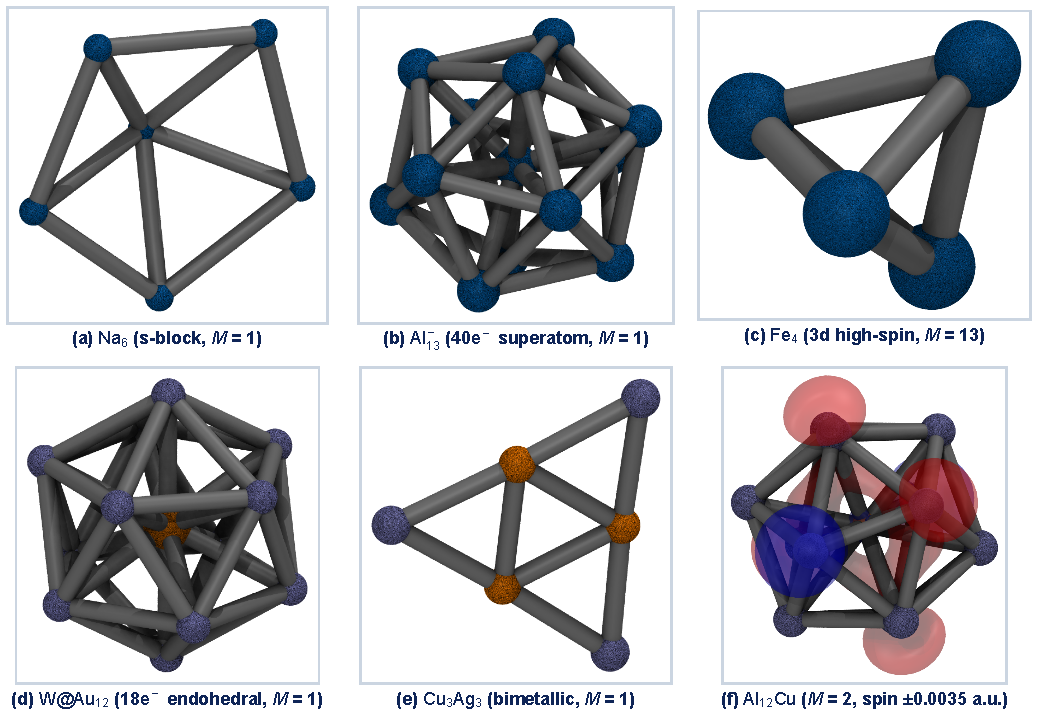
\includegraphics[width=0.92\textwidth]{figures/fig2.pdf}
  \caption{Principal-inertia-aligned 3D cluster geometries rendered via VMD (\texttt{TachyonInternal}) across six converged reference benchmarks: (a) $\mathrm{Na_6}$, (b) $\mathrm{Al_{13}^-}$, (c) $\mathrm{Fe_4}$, (d) $\mathrm{W@Au_{12}}$, (e) $\mathrm{Cu_3Ag_3}$, and (f) $\mathrm{Al_{12}Cu}$ overlaid with Multiwfn real-space spin density isosurfaces at $\pm 0.0035$~a.u. (red: $+\alpha$; blue: $-\beta$ polarization).}
  \label{fig:vmd}
\end{figure}

\begin{figure}[htbp]
  \centering
  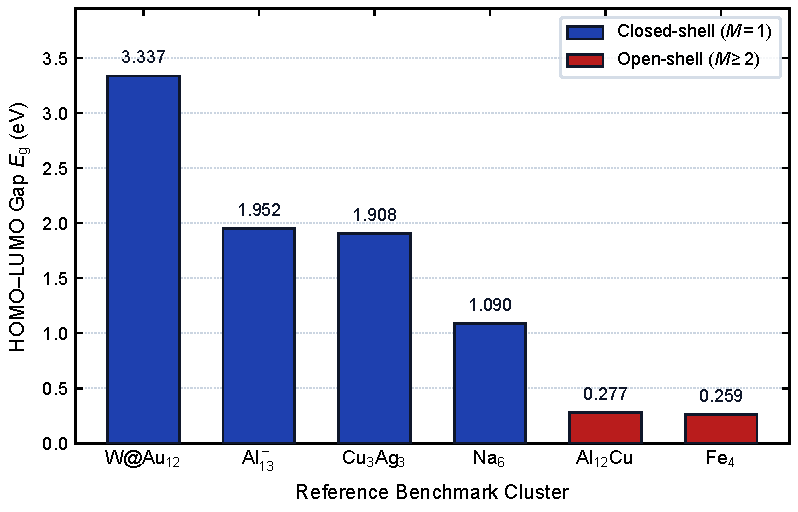
\includegraphics[width=0.72\textwidth]{figures/fig3.pdf}
  \caption{HOMO--LUMO gaps ($E_{\mathrm{g}}$, eV) across six converged reference benchmarks spanning $s$-, $p$-, $3d$-, and $5d$-block clusters (blue: closed-shell singlets $M=1$; red: open-shell magnetic/doped systems $M \ge 2$).}
  \label{fig:gaps}
\end{figure}

Across the converged systems, closed-shell superatoms $\mathrm{W@Au_{12}}$ ($18\mathrm{e}^-$, $I_h$, $E_{\mathrm{g}} = 3.337$~eV), $\mathrm{Al_{13}^-}$ ($40\mathrm{e}^-$, $1.952$~eV), and planar triangular $\mathrm{Cu_3Ag_3}$ ($1.908$~eV) exhibit wide frontier gaps, whereas high-spin $\mathrm{Fe_4}$ ($M=13$, $\langle S^2 \rangle = 42.0214$, $0.259$~eV) and doublet $\mathrm{Al_{12}Cu}$ ($M=2$, $0.277$~eV) show compressed gaps from open-shell valence manifolds. All recoverable fault injections converged autonomously, while the non-convergent SCF stress test (\texttt{fault\_scf\_noconv}) exhausted escalation safely, raised \texttt{needs\_human=True}, and surfaced severe spin contamination ($\langle S^2 \rangle = 8.4967$ vs.\ ideal $6.00$) under Article C8 as an explicit indicator of quasi-degenerate multireference character.

\subsection{$\mathrm{Al_{12}Cu}$ Multiwfn Wavefunction Analysis}

Stage S6--S7 post-processing on $\mathrm{Al_{12}Cu}$ ($q=0$, $M=2$, 37 valence electrons) resolved Hirshfeld/ADCH charges, Hirshfeld atomic spin populations, a 3,000-point PDOS spectrum ($-21.77$ to $+5.44$~eV), and frontier orbital angular-momentum compositions (Table~\ref{tab:al12cu}, Figures~\ref{fig:al12cu_elec} and~\ref{fig:al12cu_spin}). The unpaired electron delocalizes across the $\mathrm{Al_{12}}$ cage ($f_D(\mathrm{Cu}) = 3.91\%$), inducing symmetric antiparallel spin polarization ($-0.2673\,e$ and $-0.2674\,e$) on opposite aluminum vertices (\texttt{11Al}, \texttt{12Al}) that directly matches the negative $\beta$-spin lobe rendered by VMD in Figure~\ref{fig:vmd}f.

\begin{table}[htbp]
  \centering
  \caption{Quantitative Electronic and Spin Observables of $\mathrm{Al_{12}Cu}$ Extracted via Version-Locked Multiwfn 3.8(dev)}
  \label{tab:al12cu}
  \footnotesize
  \resizebox{\textwidth}{!}{%
  \begin{tabular}{@{}llll@{}}
    \toprule
    Analysis Item & Observable & Measured Value & Physical Interpretation \\
    \midrule
    Cu Charge Population & Hirshfeld / ADCH & $+0.1597\,e$ / $-0.0086\,e$ & Mild covalent hybridization between Cu and $\mathrm{Al_{12}}$ cage \\
    Hirshfeld Spin Density & $\mathrm{spin(Cu)}$ / $\sum s_i$ / $\sum |s_i|$ & $+0.0809\,e$ / $+1.0000\,e$ / $2.0694\,e$ & Net spin conserved; $f_D(\mathrm{Cu}) = 3.91\%$ (cage-delocalized) \\
    MO 93 (HOMO-$\alpha$) & Energy / $s$-$p$-$d$ (\%) / Cu (\%) & $-5.046$~eV / 18.09, 78.53, 3.37 / 17.41 & Dominated by Al $3p$ hybridized with Cu valence states \\
    MO 339 (HOMO-$\beta$) & Energy / $s$-$p$-$d$ (\%) / Cu (\%) & $-4.987$~eV / 19.45, 77.21, 3.35 / 17.68 & Symmetrical frontier character across $\alpha$/$\beta$ channels \\
    MO 94 (LUMO-$\alpha$) & Energy / $s$-$p$-$d$ (\%) / Cu (\%) & $-4.655$~eV / 24.89, 71.47, 3.65 / 15.75 & Narrow-gap open-shell acceptor (overall $E_{\mathrm{g}} = 0.277$~eV) \\
    MO 340 (LUMO-$\beta$) & Energy / $s$-$p$-$d$ (\%) / Cu (\%) & $-4.710$~eV / 20.58, 75.62, 3.80 / 16.70 & Confirms Al $3s/3p$ conduction-edge dominance \\
    \bottomrule
  \end{tabular}%
  }
\end{table}

\begin{figure}[htbp]
  \centering
  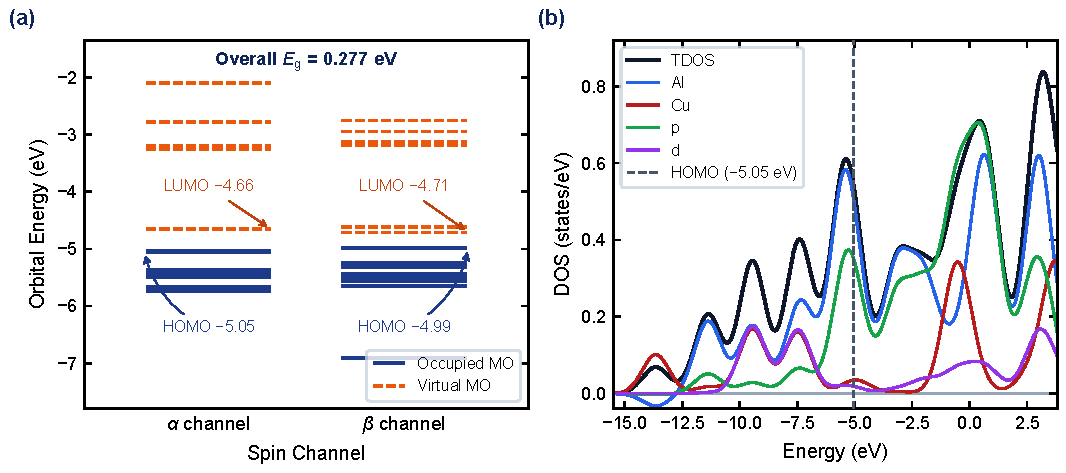
\includegraphics[width=\textwidth]{figures/fig4.pdf}
  \caption{Electronic structure of $\mathrm{Al_{12}Cu}$ ($M=2$) parsed from Gaussian 16 and Multiwfn 3.8(dev): (a) spin-polarized $\alpha$ and $\beta$ frontier molecular orbital levels (solid blue: occupied; dashed orange: virtual); (b) TDOS and Al, Cu, $p$, and $d$ projected density of states curves with vertical dashed line marking $\alpha$-HOMO ($-5.05$~eV).}
  \label{fig:al12cu_elec}
\end{figure}

\begin{figure}[htbp]
  \centering
  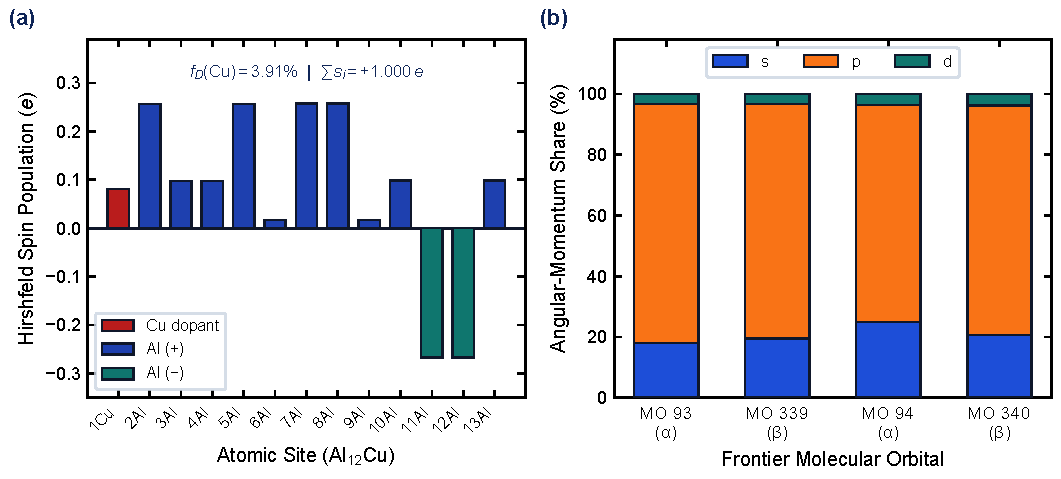
\includegraphics[width=\textwidth]{figures/fig5.pdf}
  \caption{Spin polarization and orbital bonding distribution in $\mathrm{Al_{12}Cu}$: (a) atomic Hirshfeld spin populations across all 13 sites demonstrating $f_D(\mathrm{Cu}) = 3.91\%$ and antiparallel $-0.267\,e$ polarization on \texttt{11Al}/\texttt{12Al} matching the blue isosurface lobe in Figure~\ref{fig:vmd}f; (b) $s$/$p$/$d$ angular-momentum decomposition across frontier $\alpha$/$\beta$ orbitals.}
  \label{fig:al12cu_spin}
\end{figure}

\subsection{Bilingual 50+50 Instruction Benchmark and Grounding Guard Verification}

To evaluate natural-language workflow translation without linguistic bias, the \texttt{pydantic-ai} intent planner was evaluated against two paired 50-instruction suites spanning every periodic-table block, bimetallic and endohedral doping, size-evolution ranges, charged ions, all six study recipes, three accuracy tiers, explicit time budgets, and 8 deliberately underspecified clarification prompts (\texttt{tests/llm\_eval/instructions.yaml} and \texttt{instructions\_en.yaml}). Executed live against an OpenAI-compatible DeepSeek endpoint (\texttt{deepseek-v4.1-flash}), both suites achieved 50/50 (100.0\%) accuracy (Table~\ref{tab:bilingual}).

\begin{table}[htbp]
  \centering
  \caption{Category-Level Bilingual Natural-Language-to-Plan Evaluation on \texttt{deepseek-v4.1-flash} (50 Chinese + 50 Matched English Scientific Instructions)}
  \label{tab:bilingual}
  \footnotesize
  \setlength{\tabcolsep}{4pt}
  \resizebox{\textwidth}{!}{%
  \begin{tabular}{@{}lccccc@{}}
    \toprule
    Benchmark Category & Case Count & Chinese Pass & Chinese Accuracy & English Pass & English Accuracy \\
    \midrule
    $s$-block clusters & 6 & 6/6 & 100.0\% & 6/6 & 100.0\% \\
    $p$-block clusters (incl.\ anions) & 8 & 8/8 & 100.0\% & 8/8 & 100.0\% \\
    $3d$ transition-metal \& doped & 12 & 12/12 & 100.0\% & 12/12 & 100.0\% \\
    $4d$/$5d$ \& bimetallic / endohedral & 13 & 13/13 & 100.0\% & 13/13 & 100.0\% \\
    Lanthanide ($4f$) doped & 3 & 3/3 & 100.0\% & 3/3 & 100.0\% \\
    Ambiguous (clarification required) & 8 & 8/8 & 100.0\% & 8/8 & 100.0\% \\
    \midrule
    Total & 50 & 50/50 & 100.0\% & 50/50 & 100.0\% \\
    \bottomrule
  \end{tabular}%
  }
\end{table}

On exploratory family-level prompts (such as electronic structural rigidity across heavy lanthanide endohedral gold pentamers), the planner generates concrete \texttt{ProposedPlan} entries (\texttt{Lu@Au5}, \texttt{Gd@Au5}, \texttt{Yb@Au5}) or expands the full 8-element series into independent executable projects with zero element-placeholder leakage. Offline adversarial tests in \texttt{tests/unit/test\_ai\_layer.py} verify unit-conversion equivalence pass-through, \texttt{ModelRetry} rejection of fabricated values, and UI suppression when retries exhaust.

\subsection{Autonomous Heavy Lanthanide $\mathrm{Ln@Au_5}$ Production Study}

To test unattended multi-day throughput across open-shell $4f$ clusters, an exploratory prompt initiated batch execution of all eight heavy lanthanide systems ($\mathrm{Ln@Au_5}$, $\mathrm{Ln} = \mathrm{Gd\text{--}Lu}$) alongside an independent standalone $\mathrm{Tm@Au_5}$ reproduction (\texttt{proj\_a9065c59}). Across 9 projects and 230 pipeline jobs comprising 221 Gaussian 16 calculations (18 \texttt{S0} \texttt{PBE0-D3BJ/def2-TZVP} free atoms, 184 \texttt{S3} \texttt{PBE-D3BJ/def2-SVP} isomer/multiplicity screens, and 19 \texttt{S4} three-section \texttt{--Link1--} \texttt{PBE0-D3BJ/def2-TZVP} refinements with BSE \texttt{GenECP}), the platform logged 442.76 wall-clock hours (1,399.78 CPU core-hours) and achieved 100\% convergence (230/230 jobs, 0 failures). During tail execution, elastic NUMA scaling expanded \texttt{S4} jobs from 4 cores to 10 cores (1 job) and 16 cores (2 jobs), while server-side \texttt{custodian} resolved 7 open-shell $4f$ faults autonomously (5 lossless SCF escalations across \texttt{Tb}/\texttt{Dy}/\texttt{Er}, 1 normal-mode displacement on \texttt{Tb S4 ($M=9$)}, and 1 step-limit continuation on \texttt{Dy S4 ($M=6$)}). All 19 \texttt{S4} isomers passed \texttt{n\_imag = 0} and \texttt{stable = True}.

\begin{table}[htbp]
  \centering
  \caption{Ground-State Properties (\texttt{PBE0-D3BJ/def2-TZVP}, BSE \texttt{GenECP}) and Compute Statistics Across Heavy Lanthanide $\mathrm{Ln@Au_5}$ ($\mathrm{Ln} = \mathrm{Gd\text{--}Lu}$)}
  \label{tab:lnau5}
  \scriptsize
  \setlength{\tabcolsep}{3.0pt}
  \resizebox{\textwidth}{!}{%
  \begin{tabular}{@{}llcrrcrcccc@{}}
    \toprule
    System ($Z$) & Project ID & $M_{\text{gs}}$ ($\mu_{\mathrm{B}}$) & $E_{\text{SCF}}$ (Ha) & $E_b$ (eV/at.) & $E_{\mathrm{g}}$ (eV) & $\langle S^2 \rangle$ (Ideal) & PG & $d_{\text{avg}}$(Ln--Au) (\AA) & $q_{\text{APT}}$ / spin(Ln) & Core$\cdot$h / Fixes \\
    \midrule
    $\mathrm{Gd@Au_5}$ (64) & \texttt{proj\_2c89192f} & 8 (7) & $-1444.567777$ & 1.992 & 1.679 & 15.7687 (15.75) & $C_s$ & $2.934\pm 0.107$ & $+0.44$ / $+7.74$ & 90.44 / 0 \\
    $\mathrm{Tb@Au_5}$ (65) & \texttt{proj\_19154707} & 7 (6) & $-1503.335694$ & 2.408 & 2.665 & 12.0105 (12.00) & $C_s$ & $2.827\pm 0.089$ & $+0.97$ / $+6.16$ & 109.88 / 2 \\
    $\mathrm{Dy@Au_5}$ (66) & \texttt{proj\_7a0ee451} & 6 (5) & $-1563.991806$ & 2.291 & 2.702 & 8.7572 (8.75) & $C_s$ & $2.815\pm 0.089$ & $+0.94$ / $+5.05$ & 595.42 / 3 \\
    $\mathrm{Ho@Au_5}$ (67) & \texttt{proj\_fc156187} & 5 (4) & $-1627.180455$ & 1.969 & 2.754 & 6.0000 (6.00) & $C_{2v}$ & $2.827\pm 0.160$ & $+1.15$ / $+4.10$ & 24.69 / 0 \\
    $\mathrm{Er@Au_5}$ (68) & \texttt{proj\_fa892f93} & 4 (3) & $-1694.269982$ & 2.025 & 2.709 & 3.7500 (3.75) & $C_s$ & $2.791\pm 0.080$ & $+0.92$ / $+3.06$ & 490.10 / 2 \\
    $\mathrm{Tm@Au_5}$ (69) & \texttt{proj\_735cfc68} & 3 (2) & $-1764.511111$ & 1.800 & 2.524 & 2.0000 (2.00) & $C_{2v}$ & $2.805\pm 0.150$ & $+1.11$ / $+2.04$ & 19.21 / 0 \\
    $\mathrm{Yb@Au_5}$ (70) & \texttt{proj\_51ac0f99} & 2 (1) & $-1838.137089$ & 1.802 & 1.499 & 0.7501 (0.75) & $C_s$ & $2.928\pm 0.016$ & $+0.57$ / $+0.18$ & 46.92 / 0 \\
    $\mathrm{Lu@Au_5}$ (71) & \texttt{proj\_9f91b2dc} & 1 (0) & $-1915.063709$ & 2.248 & 2.812 & --- & $C_{2v}$ & $2.782\pm 0.143$ & $+1.06$ / $0.00$ & 4.22 / 0 \\
    \bottomrule
  \end{tabular}%
  }
\end{table}

\begin{figure}[htbp]
  \centering
  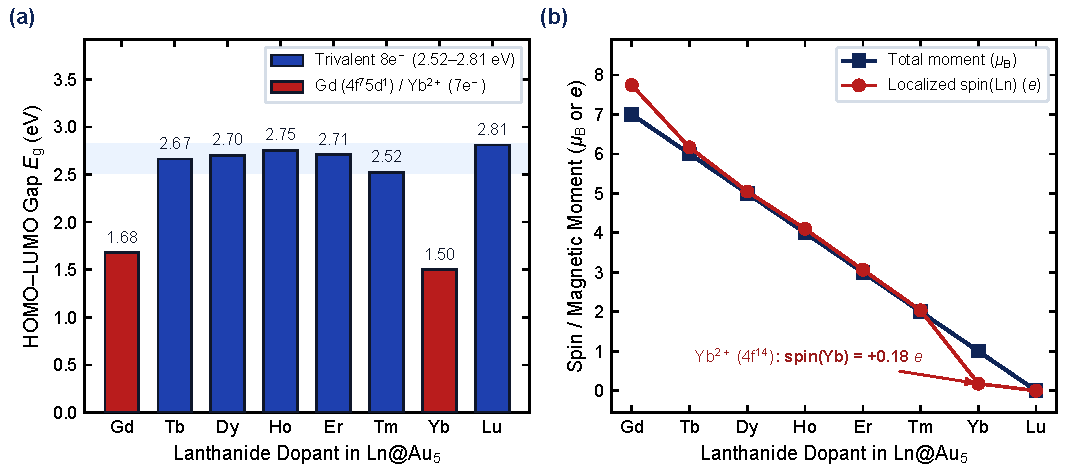
\includegraphics[width=\textwidth]{figures/fig6.pdf}
  \caption{Electronic rigidity and $4f$ spin decoupling across $\mathrm{Ln@Au_5}$ ($\mathrm{Ln} = \mathrm{Gd\text{--}Lu}$) at \texttt{PBE0-D3BJ/def2-TZVP (GenECP)}: (a) trivalent $8\mathrm{e}^-$ superatom HOMO--LUMO gap rigidity plateau ($2.524\text{--}2.812$~eV for Tb--Tm, Lu) contrasted against $\mathrm{Gd}$ ($4f^7 5d^1$) and divalent $\mathrm{Yb^{2+}}$ ($4f^{14}$, $7\mathrm{e}^-$) drops; (b) total spin magnetic moment $\mu$ ($\mu_{\mathrm{B}}$) versus localized lanthanide Mulliken spin $\mathrm{spin(Ln)}$ ($e$), confirming localized $4f$ spin behavior for Tb--Tm and abrupt spin delocalization onto the $\mathrm{Au_5}$ host in $\mathrm{Yb@Au_5}$.}
  \label{fig:lnau5}
\end{figure}

Table~\ref{tab:lnau5} and Figure~\ref{fig:lnau5} establish three distinct electronic regimes and validate single-reference fidelity across the series:
\begin{enumerate}
  \item Across Tb, Dy, Ho, Er, Tm, and Lu, trivalent $\mathrm{Ln^{3+}}$ contributes three valence electrons to the $\mathrm{Au_5}$ framework ($5 \times 1 + 3 = 8\mathrm{e}^-$ closed superatom shell), locking $E_{\mathrm{g}}$ within a rigid $2.524\text{--}2.812$~eV plateau alongside monotonic lanthanide contraction ($d_{\text{avg}}(\text{Ln--Au})$: $2.827 \rightarrow 2.782$~\AA) and high charge transfer ($q_{\text{APT}} = +0.92$ to $+1.15$).
  \item From Tb to Tm, total magnetic moment decreases monotonically ($6 \rightarrow 2\,\mu_{\mathrm{B}}$) while remaining strictly localized on the $4f$ core ($\mathrm{spin(Ln)} = +6.16 \rightarrow +2.04\,e$) with minimal spin contamination ($|\langle S^2 \rangle - S(S+1)| \le 0.0105$ across Tb--Tm, and $\le 0.0187$ across the full series), demonstrating clean electronic decoupling between core $4f^n$ spins and the $8\mathrm{e}^-$ superatom valence shell.
  \item Stabilized by the closed $4f^{14}$ subshell, $\mathrm{Yb@Au_5}$ adopts a divalent $\mathrm{Yb^{2+}}$ ($7\mathrm{e}^-$ open-shell) configuration, expanding $d_{\text{avg}}(\text{Yb--Au})$ to $2.928$~\AA, lowering $q_{\text{APT}}$ to $+0.57$, collapsing $E_{\mathrm{g}}$ to $1.499$~eV, and delocalizing the unpaired spin onto the $\mathrm{Au_5}$ framework (only $+0.18\,e$ on Yb). Independent reproduction \texttt{proj\_a9065c59} ($\mathrm{Tm@Au_5}$, $E_{\text{SCF}} = -1764.510373$~Ha, $E_{\mathrm{g}} = 2.521$~eV) matches batch project \texttt{proj\_735cfc68} within $0.0007$~Ha and $0.003$~eV.
\end{enumerate}
While Article C8 propagates \texttt{rule.f\_block.experimental\_warning} across all lanthanide runs to alert users where multireference (CASSCF/CASPT2) or spin-orbit relativistic treatments are required for excited-state multiplet splittings, the vanishing $\langle S^2 \rangle$ deviations ($\le 0.019$) and verified \texttt{stable=opt} minima confirm that broken-symmetry hybrid DFT captures the ground-state superatom shell closures, geometric contraction, and divalent $\mathrm{Yb^{2+}}$ transition with quantitative consistency.

\subsection{Five-Tier Verification and Interactive Workbench}

QuantumChem AI comprises 75 Python modules under \texttt{src/} and 11 Streamlit modules under \texttt{web/}, backed by a five-tier verification pyramid (Table~\ref{tab:tests}). All source files pass \texttt{ruff} linting and formatting, strict \texttt{mypy src} type checking, AST zero-element-branch auditing, and 115 offline unit and headless Playwright E2E browser tests. The six-view web and desktop workbench (\texttt{qcai web} and \texttt{qcai-app}) unifies periodic-table/natural-language study setup (Figure~\ref{fig:ui}a), auditable plan confirmation, server telemetry, and an interactive results dashboard (Figure~\ref{fig:ui}b) with CSV export, Origin/VMD rendering controls, and A4 PDF report generation.

\begin{table}[htbp]
  \centering
  \caption{Five-Tier Automated Verification Pyramid of QuantumChem AI}
  \label{tab:tests}
  \footnotesize
  \resizebox{\textwidth}{!}{%
  \begin{tabular}{@{} >{\raggedright\arraybackslash}p{2.3cm} >{\raggedright\arraybackslash}p{4.7cm} >{\raggedright\arraybackslash}p{3.3cm} >{\raggedright\arraybackslash}p{3.9cm} @{}}
    \toprule
    Tier & Verification Scope & Observed Status & Representative Modules / Gates \\
    \midrule
    L1: Static \& Constitution & \texttt{ruff}, \texttt{mypy src}, AST 0-element check, \texttt{Hypothesis} tests & 75 files typed; 0 AST violations & \texttt{test\_axiom\_no\_\allowbreak{}element\_\allowbreak{}branches.py} \\
    L2: Offline Unit & Energetics, SCF/tail repair, BSE \texttt{GenECP}, 3-axis dedup, guards & 115 offline tests passed & \texttt{tests/unit/*.py} \\
    L3: Local Renderers & Origin 2024b (incl.\ \texttt{PAN4}, $\mathrm{Ln@Au_5}$) \& VMD ray tracing & 6 Origin tests + VMD render passed & \texttt{test\_origin\_\allowbreak{}renderer.py} \\
    L4: HPC \& Live AI & Linux SSH probe, 10 reference runs, 230-job $\mathrm{Ln@Au_5}$, 50+50 eval & 100\% converged; 50/50 ZH \& 50/50 EN & \texttt{test\_remote\_ssh.py}, \texttt{test\_deepseek\_llm.py} \\
    L5: Browser E2E & Playwright Chromium 6-page workflow + CLI help & All E2E \& CLI tests passed & \texttt{tests/e2e/\allowbreak{}test\_web\_flow.py} \\
    \bottomrule
  \end{tabular}%
  }
\end{table}

\begin{figure}[htbp]
  \centering
  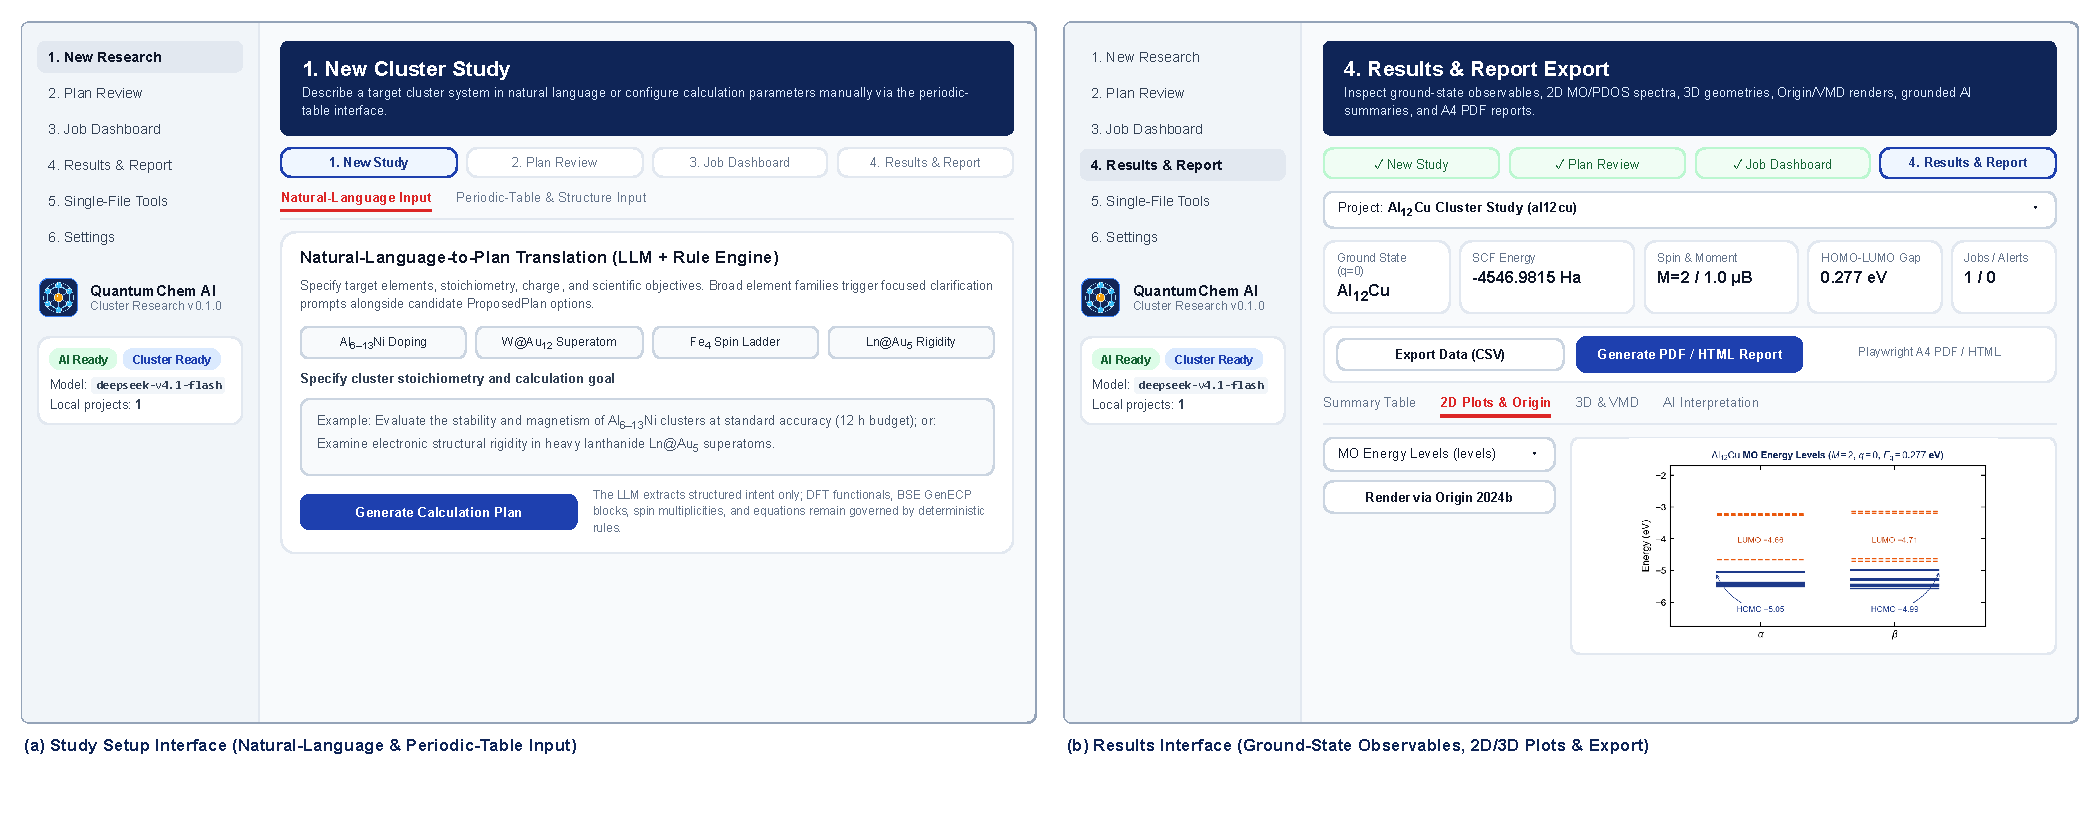
\includegraphics[width=\textwidth]{figures/fig7.pdf}
  \caption{QuantumChem AI interactive web workbench: (a) study setup view supporting natural-language and periodic-table input; (b) results view displaying ground-state summary metrics for $\mathrm{Al_{12}Cu}$, CSV/PDF export controls, and 2D MO/PDOS, 3D geometry, and guarded AI analysis tabs.}
  \label{fig:ui}
\end{figure}

\section{Conclusions}

QuantumChem AI establishes a reproducible, rule-governed electronic-structure workflow methodology spanning the periodic table for atomic cluster research. Enforcing the eight-article Design Constitution (C1--C8) through AST static checks, Basis Set Exchange \texttt{Gen}/\texttt{GenECP} coverage verification (covering built-in \texttt{def2}, augmented \texttt{ma-def2}, and scalar-relativistic \texttt{SARC-DKH2}/\texttt{DKH2} specifications), tri-axial inertia Kabsch deduplication, three-section \texttt{--Link1--} stability checks, lossless $4f$/tail recovery, and unit-aware LLM grounding eliminates element-specific hardcoding and unverified AI claims while maintaining 100.0\% (50/50 Chinese and 50/50 English) planning accuracy. Validated across 10 Gaussian 16 reference benchmarks, $\mathrm{Al_{12}Cu}$ wavefunction spectroscopy, and an autonomous 230-job (1,399.78 CPU core-hours, 100\% convergence) campaign on $\mathrm{Ln@Au_5}$ ($\mathrm{Ln} = \mathrm{Gd\text{--}Lu}$), the platform provides both resilient HPC automation and quantitative insight into trivalent $8\mathrm{e}^-$ superatom gap rigidity, localized $4f$ spin decoupling, and divalent $\mathrm{Yb^{2+}}$ electronic transitions.

\section*{Data and Software Availability}

The complete source code of QuantumChem AI is openly released under the MIT License (\texttt{LICENSE}) at \url{https://github.com/QIANCHANGKING/quantumchem-ai} and permanently archived on Zenodo under DOI \texttt{10.5281/zenodo.24501860}. The package targets Python 3.12 (dependency-locked via \texttt{pyproject.toml} and \texttt{uv.lock}) and operates on Windows 10/11 (desktop UI, Origin 2024b, VMD, and Chromium PDF generation) and Linux x86\_64 (remote HPC worker execution). All 115 offline unit, AST constitutional-gate, reference benchmark regression, and Playwright E2E tests execute without external HPC access or API credentials.

External computational and visualization programs orchestrated by QuantumChem AI are available from their respective providers: Gaussian 16 (Rev.\ C.02, \url{https://gaussian.com}), Multiwfn 3.8(dev) (\url{http://sobereva.com/multiwfn/}), Origin 2024b (\url{https://www.originlab.com}), VMD (\url{https://www.ks.uiuc.edu/Research/vmd/}), and ABCluster / GFN2-xTB (\texttt{tblite}). All reference Gaussian 16 logs (\texttt{tests/data/golden/}), Multiwfn outputs (\texttt{tests/data/multiwfn/al12cu/}), $\mathrm{Ln@Au_5}$ summary datasets (\texttt{paper/data/ln\_au5\_summary.json} and \texttt{results/ln\_au5\_study/}), and bilingual 50+50 instruction suites (\texttt{tests/llm\_eval/instructions.yaml} and \texttt{instructions\_en.yaml}) are included in the repository and Supporting Information.

\begin{suppinfo}
Supporting Information provides: (S1) offline installation and 115-test verification guide; (S2) complete YAML rule-engine specification tables; (S3) complete 10-benchmark and 19-isomer $\mathrm{Ln@Au_5}$ ($\mathrm{Gd\text{--}Lu}$) quantitative tables, 7 server-side \texttt{custodian} recovery traces, and optimized Cartesian coordinates (\AA); and (S4) category-level 50+50 bilingual natural-language instruction evaluation breakdown.
\end{suppinfo}

\begin{acknowledgement}
The author thanks the local Linux compute cluster administrators for computational resources supporting the multi-day $\mathrm{Ln@Au_5}$ production campaign.
\end{acknowledgement}

\section*{Author Information}
Changtian Qian: ORCID \url{https://orcid.org/0009-0005-2464-3814}.

\section*{Notes}
The author declares no competing financial interest.

\bibliography{references}

\begin{tocentry}
  \centering
  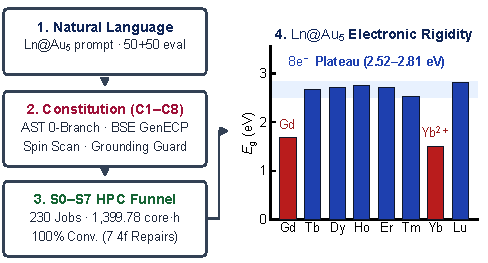
\includegraphics[width=3.20in,height=1.72in,keepaspectratio]{figures/TOC_graphic.pdf}
\end{tocentry}

\end{document}
